\documentclass[12pt,a4paper]{beamer}
\usepackage[utf8]{inputenc}
\usepackage{amsmath}
\usepackage{amsfonts}
\usepackage{amssymb, multicol}
\usepackage{framed}

\usepackage{graphicx}
\usepackage{caption}
\usepackage{subcaption}

\begin{document}
\begin{frame}{Numerical variables inference}
	\begin{itemize}
		\item Are books cheaper online?
		\item Do men run, on average, faster than women?
		\item Is the average weights of chickens that were fed linseed, sunflower and soybean different?
	\end{itemize}
\end{frame}
\begin{frame}{Numerical inference}
	\textbf{Paired data}\\
	Two sets of observations are \emph{paired} if each observation in one set has a special correspondence or connection with exactly one observation in the other data set.
\end{frame}
\begin{frame}{Paired data}
	Prices of textbooks at UCLA's bookstore and Amazon.com
	\begin{table}[h]
	\centering
	\resizebox{0.7\textwidth}{!}{
	\begin{tabular}{rllrrr}
	  \hline
	 & dept & course & ucla & amazon & diff \\ 
	  \hline
	1 & Am Ind &  C170 & 27.67 & 27.95 & -0.28 \\ 
	  2 & Anthro & 9 & 40.59 & 31.14 & 9.45 \\ 
	  3 & Anthro & 135T & 31.68 & 32.00 & -0.32 \\ 
	  4 & Anthro & 191HB & 16.00 & 11.52 & 4.48 \\ 
	$\vdots$ & $\vdots$ & $\vdots$ & $\vdots$ & $\vdots$ & $\vdots$ \\
	  72 & Wom Std & M144 & 23.76 & 18.72 & 5.04 \\ 
	  73 & Wom Std & 285 & 27.70 & 18.22 & 9.48 \\ 
	   \hline
	\end{tabular}}
	\end{table}
	where $diff=UCLA-Amazon$ is the price difference.
\end{frame}
\begin{frame}{Paired data}
	\textbf{Hypothesis testing}
	\begin{itemize}
	\setlength{\itemsep}{0mm}
	\item[$H_0$:] $\mu_{diff}=0$. There is no difference in the average textbook price.
	\item[$H_A$:] $\mu_{diff} \neq 0$. There is a difference in average prices.
	\end{itemize}
	\textbf{Test statistic:}
	\[Z=\frac{\mu_{diff}-0}{SE_{diff}},\]
	where $SE_{diff}=\frac{se_{diff}}{\sqrt{n_{diff}}}.$
\end{frame}
\begin{frame}{Paired data}
	Summary statistics for the price differences.
	\begin{table}[hh]
	\centering
	\begin{tabular}{ccccc}
	\hline
	$n_{_{diff}}$	&\hspace{3mm}& $\bar{x}_{_{diff}}$	&\hspace{3mm}& $s_{_{diff}}$ \vspace{1mm}\\
	73			&& 12.76				&& 14.26 \\
	\hline
	\end{tabular}

	\end{table}
\textbf{Test statistic:}
\[Z =\frac{12.76 - 0}{1.67} = 7.59\]
\textbf{p-value}
\[p-value=P(|Z|>7.59)=2P(Z>7.59)=0.0004\]
Since $p-value$ is smaller than $\alpha=0.05$ we reject the null hypothesis.  We have found 
convincing evidence that Amazon prices are different from the UCLA prices for textbooks. 

\end{frame}
\begin{frame}{Difference in mean}
	\[\textbf{Compering group averages}\]
	The Cherry Blossom run... yet again...
	\begin{table}[h]
	\centering
	\begin{tabular}{l rr}
	\hline
		&	men	&	women \\
	\hline
	$\bar{x}$	& 87.65	& 102.13 \\
	$s$	&	12.5		& 15.2 \\
	$n$	&	45		& 55    \\
	\hline
	\end{tabular}
	
	\end{table}
\end{frame}
\begin{frame}{Difference in mean}
	\textbf{Hypothesis testing}
	\begin{itemize}
	\setlength{\itemsep}{0mm}
	\item[$H_0$:] $\mu_m-\mu_w=0$. There is no difference between the average running time of men and women
	\item[$H_A$:] $\mu_{m}-\mu_{w} \neq 0$. There is a difference in average running time.
	\end{itemize}
	\textbf{Test statistic:}
	\[Z=\frac{\mu_m-\mu_w-0}{SE_{\bar{x}_{m} - \bar{x}_{w}}},\]
	where 
	\begin{eqnarray}
	SE_{\bar{x}_{m} - \bar{x}_{w}} = \sqrt{\frac{s_m^2}{n_m} + \frac{s_w^2}{n_w}}
	\end{eqnarray}
		\textbf{Confidence interval}
		\[\mu_m-\mu_w\pm z^*SE_{\bar{x}_m-\bar{x}_w}\]
\end{frame}
\begin{frame}{Difference in mean}
	\textbf{Conditions for normality}
	\begin{itemize}
	\item The sample means, $\bar{x}_m$ and $\bar{x}_w$, each meet the criteria for having nearly normal sampling distributions.
	\item The observations in the two samples are independent.
\end{itemize}
\end{frame}
\begin{frame}{Difference in mean}
	\textbf{Test statistic:}
	\[Z =\frac{14.48}{2.77} = 75.69\]
	\textbf{p-value}
	\[p-value=P(|Z|>75.69)=2P(Z>75.59)\simeq 0\]
	Since p-value is almost zero we reject the null hypothesis. 
\textbf{ 95\% Confidence interval}
\[14.48\pm 1.96\cdot 2.77=(9.05,19.9)\]
\end{frame}
\begin{frame}{The normality condition}
	\textbf{Reminder:}\\
	Important conditions to help ensure the sampling distribution of $\bar{x}$ is nearly normal and the estimate of SE sufficiently accurate:
	\begin{itemize}
	\setlength{\itemsep}{0mm}
	\item The sample observations are independent.
	\item The sample size is large: $n\geq30$ is a good rule of thumb.
	\item The population distribution is not strongly skewed. 
	\end{itemize}\vspace{0.3cm}
	\textbf{Q} What if we have a small sample? $n<30.$
\end{frame}
\begin{frame}{T-distirbution}
	\textbf{T-distribution vs. Normal distibution}
	\begin{figure}
	\centering
	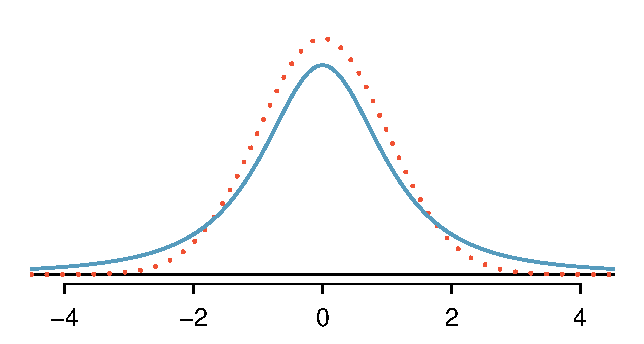
\includegraphics[height=45mm]{figures/tDistCompareToNormalDist/tDistCompareToNormalDist}
	\caption{Comparison of a $t$ distribution (solid line) and a normal distribution (dotted line).}
	\end{figure}
\end{frame}
\begin{frame}{T-distribution}
	\textbf{Degrees of freedom (df)}\\
	The degrees of freedom describe the shape of the $t$ distribution. The larger the degrees of freedom, the more closely the distribution approximates the normal model.
	\begin{figure}
	\centering
	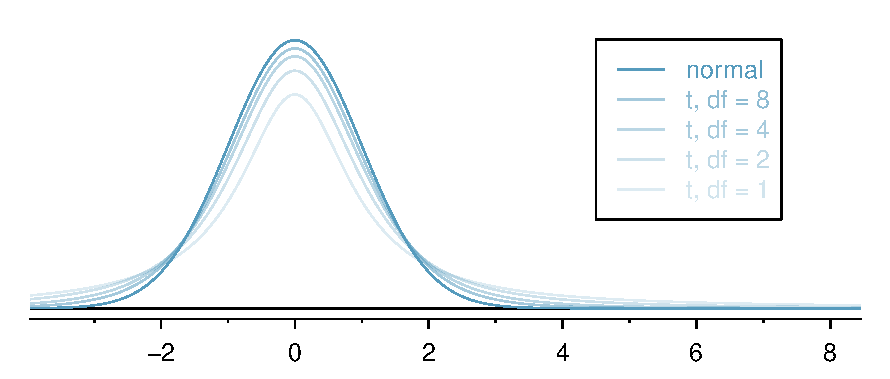
\includegraphics[width=0.8\textwidth]{figures/tDistConvergeToNormalDist/tDistConvergeToNormalDist}
	\end{figure}
\end{frame}
\begin{frame}{T-distribution}
	\begin{table}[hht]
	\centering
	\resizebox{0.5\textwidth}{!}{
	\begin{tabular}{r | rrr rr}
	one tail & \hspace{1.5mm}  0.100 & \hspace{1.5mm} 0.050 & \hspace{1.5mm} 0.025 & \hspace{1.5mm} 0.010 & \hspace{1.5mm} 0.005  \\
	two tails & 0.200 & 0.100 & 0.050 & 0.020 & 0.010 \\
	\hline
	{$df$} \hfill 1  &  {\normalsize  3.08} & {\normalsize  6.31} & {\normalsize 12.71} & {\normalsize 31.82} & {\normalsize 63.66}  \\ 
	2  &  {\normalsize  1.89} & {\normalsize  2.92} & {\normalsize  4.30} & {\normalsize  6.96} & {\normalsize  9.92}  \\ 
	3  &  {\normalsize  1.64} & {\normalsize  2.35} & {\normalsize  3.18} & {\normalsize  4.54} & {\normalsize  5.84}  \\ 
	$\vdots$ & $\vdots$ &$\vdots$ &$\vdots$ &$\vdots$ & \\
	17  &  {\normalsize  1.33} & {\normalsize  1.74} & {\normalsize  2.11} & {\normalsize  2.57} & {\normalsize  2.90}  \\ 
	\textbf{18}  &  \textbf{\normalsize  1.33} & \textbf{\normalsize  1.73} & \textbf{\normalsize  2.10} & \textbf{\normalsize  2.55} & \textbf{\normalsize  2.88}  \\ 
	19  &  {\normalsize  1.33} & {\normalsize  1.73} & {\normalsize  2.09} & {\normalsize  2.54} & {\normalsize  2.86}  \\ 
	20  &  {\normalsize  1.33} & {\normalsize  1.72} & {\normalsize  2.09} & {\normalsize  2.53} & {\normalsize  2.85}  \\ 
	$\vdots$ & $\vdots$ &$\vdots$ &$\vdots$ &$\vdots$ & \\
	400  &  {\normalsize  1.28} & {\normalsize  1.65} & {\normalsize  1.97} & {\normalsize  2.34} & {\normalsize  2.59}  \\ 
	500  &  {\normalsize  1.28} & {\normalsize  1.65} & {\normalsize  1.96} & {\normalsize  2.33} & {\normalsize  2.59}  \\ 
	$\infty$  &  {\normalsize  1.28} & {\normalsize  1.64} & {\normalsize  1.96} & {\normalsize  2.33} & {\normalsize  2.58}  \\ 
	\end{tabular}}
	\end{table}
	\begin{figure}
	\centering
	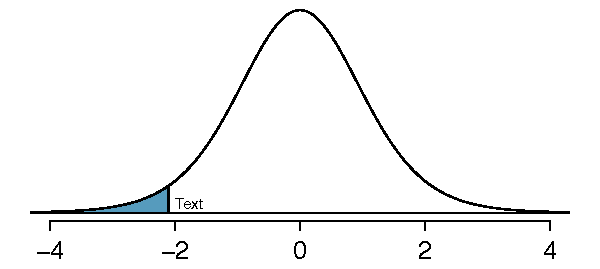
\includegraphics[width=0.55\textwidth]{figures/tDistDF18LeftTail2Point10/tDistDF18LeftTail2Point10}
	\end{figure}
\end{frame}
\begin{frame}{T-distribution}
	\begin{itemize}
	\item \textbf{Independence of observations.}
	
	 We verify this condition just as we did before. We collect a simple random sample from less than 10\% of the population, or if it was an experiment or random process, we carefully check to the best of our abilities that the observations were independent.
	\item \textbf{Observations come from a nearly normal distribution.}
	
	 This second condition is difficult to verify with small data sets. We often (i) take a look at a plot of the data for obvious departures from the normal model, and (ii) consider whether any previous experiences alert us that the data may not be nearly normal.
	\end{itemize}
\end{frame}
\begin{frame}{Inference for $\bar{x}$}
	\begin{itemize}
		\item  \textbf{Degrees of freedom:} $df=n-1,$ where $n$ is the number of observations
		\vspace{0.3cm}
		\item \textbf{Confidence interval:}
		\[\bar{x} \ \pm\  t^{\star}_{df}SE\]

		.
	\end{itemize}
	

\end{frame}
\begin{frame}{Inference for $\bar{x}$}
	 \textbf{Hypothesis testing}
			\small\begin{itemize}
			\setlength{\itemsep}{0mm}
			\item[$H_0$:] $\mu = \mu_0$.
			\item[$H_A$:]$\left\{
			\begin{array}{ll}
				\mu>\mu_0& \text{(upper-tail alternative)}\\
				\mu\neq\mu_0& \text{(two-tailed alternative)}\\
				\mu< \mu_0& \text{(lower-tail alternative)}
			\end{array}
			\right.$
		\end{itemize}
		Test statistic: $t=\frac{\bar{x}-\mu_0}{SE}$\\
		We reject $H_0$ when:
		\begin{itemize}
			\item $P(T_{df}>t)<\alpha$ (upper-tail alternative)
			\item $P(|T_{df}|>t)<\alpha$ (two-tailed alternative)
			\item $P(T_{df}<-t)<\alpha$ (lower-tail alternative)
	\end{itemize}
\end{frame}
\begin{frame}{Paired data for small sample}
	\begin{itemize}
		\item  \textbf{Degrees of freedom:} $df=n-1,$ where $n$ is the number of observations
		\vspace{0.3cm}
		\item \textbf{Confidence interval:}
		\[\bar{x}_{diff} \ \pm\  t^{\star}_{df}SE_{diff}\]

		.
	\end{itemize}
	

\end{frame}
\begin{frame}{Paired data for small sample}
	\textbf{Hypothesis testing}
	\begin{itemize}
	\setlength{\itemsep}{0mm}
	\item[$H_0$:] $\mu_{diff}=0$. 
	\item[$H_A$:] $\mu_{diff} \neq 0$. 
	\end{itemize}
	\textbf{Test statistic:}
	\[T=\frac{\mu_{diff}-0}{SE_{diff}},\]
	where $SE_{diff}=\frac{se_{diff}}{\sqrt{n_{diff}}}.$
\end{frame}
\begin{frame}{Difference in mean for small samples}
	\begin{itemize}
		\item  \textbf{Degrees of freedom:} $df=\min\{n_1-1,n_2-1\},$ where $n_1,n_2$ is the number of observations in the respective groups.
		\vspace{0.3cm}
		\item \textbf{Confidence interval:}
		\[\bar{x}_1-\bar{x}_2 \ \pm\  t^{\star}_{df}SE_{diff},\]
		where 
		\begin{eqnarray}
		SE_{\bar{x}_{1} - \bar{x}_{2}} = \sqrt{\frac{s_1^2}{n_1} + \frac{s_2^2}{n_2}}
		\end{eqnarray}
	\end{itemize}
\end{frame}
\begin{frame}{Difference in mean for small samples}
	\begin{itemize}
		\item\textbf{Hypothesis testing}
	\begin{itemize}
	\setlength{\itemsep}{0mm}
	\item[$H_0$:] $\mu_1-\mu_2=0$. 
	\item[$H_A$:] $\mu_{1}-\mu_{2} \neq 0$. 
	\end{itemize}
	\item\textbf{Test statistic:}
	\[T=\frac{\mu_1-\mu_2-0}{SE_{\bar{x}_{m} - \bar{x}_{w}}},\]
	\end{itemize}
	\end{frame}
\begin{frame}{Difference in mean for small samples}
	\textbf{Conditions }
	\begin{itemize}
	\item Each sample meets the criteria for using the $t$ distribution.
	\item The samples are independent.
\end{itemize}
\end{frame}
\begin{frame}{Example}
	\begin{itemize}
	\item An SAT preparation company claims that its students' scores improve by over 100 points on average after their course.
	\item We have a random sample of the scores of $30$ students, before and after.
	\item Which test should we apply to check is the companies claim is true?
\end{itemize}
\end{frame}
\begin{frame}{T-student difference test}
	\begin{itemize}
		\item Calculate the difference in scores for each student; $x_i$ denotes the difference for the $i$th student.
		\item Check the conditions:
		\begin{itemize}
			\item Independence holds.
			\item Approximately normal
				\end{itemize}
			\end{itemize}
			\begin{figure}[h]
			\centering
			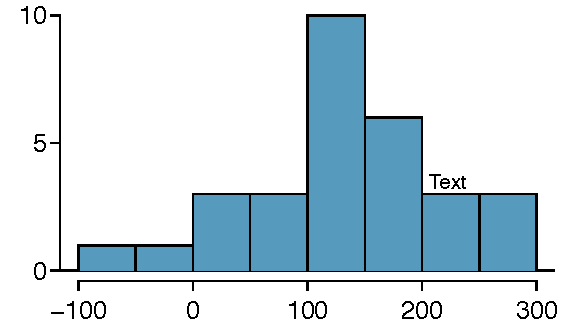
\includegraphics[width=0.54\textwidth]{figures/satImprovementHTDataHistogram/satImprovementHTDataHistogram}
			\end{figure}
	
\end{frame}
\begin{frame}{T-student difference test}
	\begin{itemize}
		\item $H_0$: student scores do not improve by more than 100 after taking the company's course. 
		\item  $H_A$: students scores improve by more than 100 points on average after taking the company's course. 
	\end{itemize}
	\textbf{Or}
	\begin{itemize}
		\item	$H_0:\mu_{_{diff}} = 100$ 
		\item $H_A:\mu_{_{diff}} > 100$.
	\end{itemize}
\end{frame}
\begin{frame}{T-student difference test}
	\begin{table}[h]
	\centering
	\begin{tabular}{ccc}
	\hline
	$n$ & $\bar{x}$ & $s$  \\
	30   & 135.9	  & 82.2 \\
	\hline
	\end{tabular}
	\end{table}
	\begin{itemize}
		\item $df=n-1=29$
		\vspace{0.3cm}
		\item  $t=\frac{\bar{x}-100}{SE_{diff}}=\frac{135.9-133}{82/\sqrt{30}}=2.39$
		\item $p-value=P(T>t)=0.0118<0.05=\alpha$
		\item We reject the null hypothesis. The data provide convincing evidence to support the company's claim that student scores improve by more than 100 points following the class.
	\end{itemize}
\end{frame}
\begin{frame}{Comparing many means}
	\begin{itemize}
		\item What is we want to compare means from $k$ groups, with $k>2$?
		\item We have the following hypothesis test: 
		\begin{itemize}
		\setlength{\itemsep}{0mm}
		\item [$H_0$:]The mean outcome is the same across all groups.
		\item [$H_A$:] At least one mean is different.
		\end{itemize}
		\textbf{Or}
		\begin{itemize}
			\setlength{\itemsep}{0mm}
			\item [$H_0$:]$\mu_1 = \mu_2 = \cdots = \mu_k$
			\item [$H_A$:] At least one mean is different.
			\end{itemize}
	\end{itemize}
\end{frame}
\begin{frame}{ANOVA}
	\textbf{Batting average}
	\begin{table}[h]
	\centering
	\resizebox{0.7\textwidth}{!}{
	\begin{tabular}{rlllrrrrrr}
	  \hline
	 & name & team & position & AB & H & HR &RBI & AVG & OBP \\ 
	  \hline
	1 & I Suzuki & SEA & OF & 680 & 214 & 6 & 43 & 0.315 & 0.359 \\ 
	  2 & D Jeter & NYY & IF & 663 & 179 & 10 & 67 & 0.270 & 0.340 \\ 
	  3 & M Young & TEX & IF & 656 & 186 & 21 & 91 & 0.284 & 0.330 \\ 
	  $\vdots$ & $\vdots$ & $\vdots$ & $\vdots$ & $\vdots$ & $\vdots$ & $\vdots$ & $\vdots$ \\
	  325 & B Molina & SF & C & 202 & 52 & 3 & 17 & 0.257 & 0.312 \\ 
	  326 & J Thole & NYM & C & 202 & 56 & 3 & 17 & 0.277 & 0.357 \\ 
	  327 & C Heisey & CIN & OF & 201 & 51 & 8 & 21 & 0.254 & 0.324 \\ 
	   \hline
	\end{tabular}}
	\end{table}
	\begin{table}[h]
	\centering
	\resizebox{0.6\textwidth}{!}{
	\begin{tabular}{lp{8.5cm}}
	\hline
	{\bf variable} & {\bf description} \\
	\hline
	name & Player name \\
	team & The abbreviated name of the player's team \\
	position & The player's primary field position (OF, IF, DH, C) \\
	AB & Number of opportunities at bat \\
	H & Number of hits \\
	HR & Number of home runs \\
	RBI & Number of runs batted in \\
	AVG & Batting average, which is equal to $H/AB$ \\
	OBP & On-base percentage, which is roughly equal to the fraction of times a player gets on base or hits a home run \\
	\hline
	\end{tabular}}
	\end{table}
\end{frame}
\begin{frame}{ANOVA}
	\begin{figure}
	\centering
	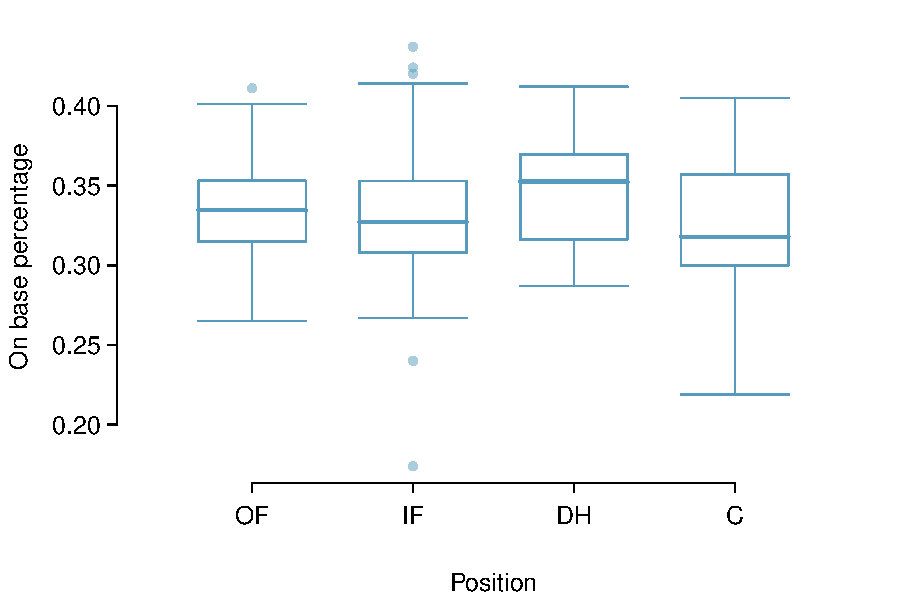
\includegraphics[width=0.6\textwidth]{figures/mlbANOVA/mlbANOVABoxPlot}
	\end{figure}
	\textbf{Summary statistics}
	\begin{table}[ht]
	\centering
	\resizebox{0.7\textwidth}{!}{
	\begin{tabular}{lrrrr}
	\hline
		& OF & IF & DH & C \\
	\hline
	Sample size ($n_i$)	& 120 & 154 & 14 & 39 \\
	Sample mean ($\bar{x}_i$)	& 0.334 & 0.332 & 0.348 & 0.323 \\
	Sample SD ($s_i$)	& 0.029 & 0.037 & 0.036 & 0.045 \\
	\hline
	\end{tabular}}
	\end{table}
\end{frame}
\begin{frame}{ANOVA}
	\textbf{Hypothesis}
	\begin{itemize}
	\setlength{\itemsep}{0mm}
	\item $H_0:$ $\mu_{OF} = \mu_{IF} = \mu_{DH} = \mu_{C}$
	\item $H_A:$ The average on-base percentage ($\mu_i$) varies across some (or all) groups.
	\end{itemize}
\end{frame}
\begin{frame}{ANOVA}
	\textbf{Preliminary}\\
		\textbf{Mean square between groups ($MSG$)} for $k$ groups.
		\begin{align*}
		MSG = \frac{1}{df_{G}}SSG = \frac{1}{k-1}\sum_{i=1}^{k} n_{i}\left(\bar{x}_{i} - \bar{x}\right)^2
		\end{align*}
		where $SSG$ is called the \textbf{sum of squares between groups} and $n_{i}$ is the sample size of group $i$. $MSG$ has $df_{G}=k-1$.
\end{frame}
\begin{frame}{ANOVA}
	\small\begin{itemize}
%\item	\textbf{Sum of squares total ($SST$)} is computed as
%	\begin{align*}
%	SST = \sum_{i=1}^{n} \left(x_{i} - \bar{x}\right)^2
%	\end{align*}
\item \textbf {Sum of squared errors ($SSE$)} in one of two equivalent ways:
	\begin{align*}
	SSE&= (n_1-1)s_1^2 + (n_2-1)s_2^2 + \cdots + (n_k-1)s_k^2
	\end{align*}
	where $s_i^2$ is the sample variance in group $i$. 
	\item \textbf{ Mean Square Error ($MSE$)} \\
	 \[MSE = \frac{1}{df_{E}}SSE,\]
	where $df_{E}=n-k$ and $n$ is the total sample size.
	\end{itemize}
\end{frame}
\begin{frame}{ANOVA}
	\textbf{Test statistic}
	\[F=\frac{MSG}{MSE},\]
	\textbf{F-distribution} with degrees of freedom $(df_1,df_2)=(k-1,n-k).$
\end{frame}
\begin{frame}
	\textbf{Bating average Hypothesis}
	\[F= 1.994,\text{ with }(df_G,df_E)=(3,323)\]
	\begin{figure}[ht]
	\centering
	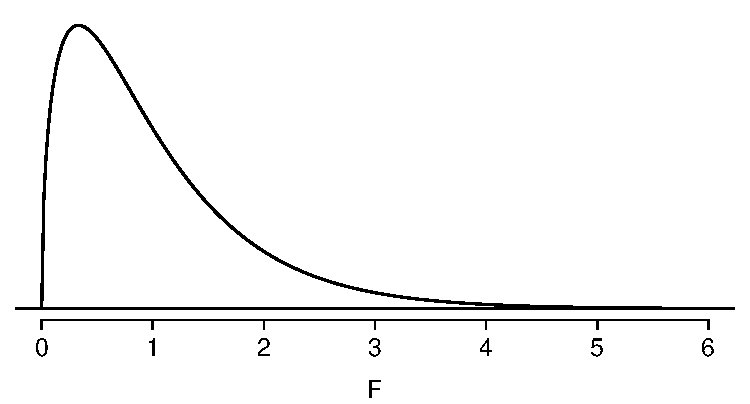
\includegraphics[width=0.7\textwidth]{figures/fDist3And323/fDist3And323}
	
	\end{figure}
$p-value=0.115$
\end{frame}
\begin{frame}{ANOVA}
	\textbf{ANOVA Summary Table}
	\begin{table}[ht]
	\centering
	\begin{tabular}{lrrrrr}
	  \hline
	 & Df & Sum Sq & Mean Sq & F value & Pr($>$F) \\ 
	  \hline
	position & 3 & 0.0076 & 0.0025 & 1.9943 & 0.1147 \\ 
	  Residuals & 323 & 0.4080 & 0.0013 &  &  \\    \hline
	\multicolumn{6}{r}{$s_{pooled} = 0.036$ on $df=323$}
	\end{tabular}

	\label{anovaSummaryTableForOBPAgainstPosition}
	\end{table}
\end{frame}
\begin{frame}{ANOVA}
	\textbf{Conditions}
	\begin{itemize}
		\item Independence
		\item Approximately normal
		\item Constant variance: the variance in the groups is about equal from one group to the next.
	\end{itemize}
		
\end{frame}
\begin{frame}{ANOVA}
	\begin{figure}[hhh]
	\centering
	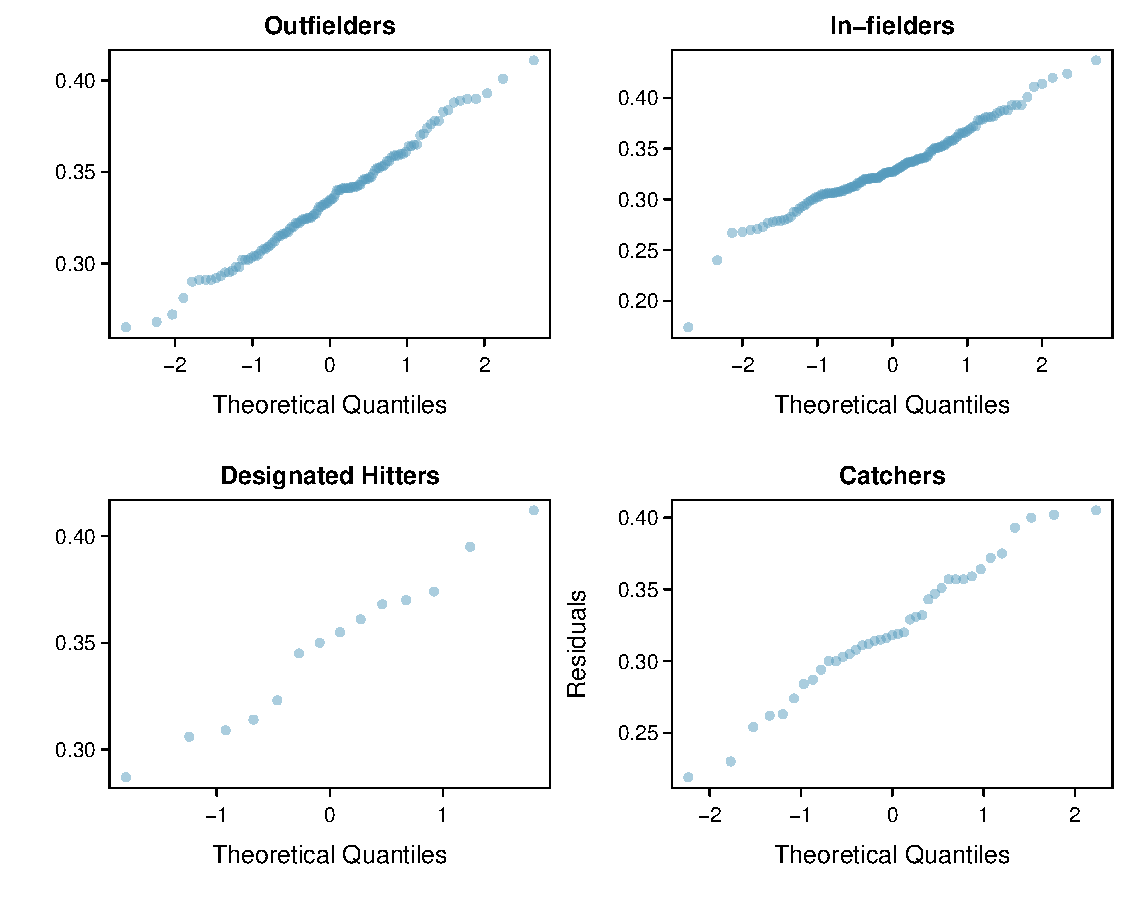
\includegraphics[width=0.7\textwidth]{figures/mlbANOVA/mlbANOVADiagNormalityGroups}
	\end{figure}
\end{frame}
\begin{frame}{ANOVA}
	\begin{table}[ht]
	\centering
	\resizebox{0.7\textwidth}{!}{
	\begin{tabular}{lrrrr}
	\hline
		& OF & IF & DH & C \\
	\hline
	Sample size ($n_i$)	& 120 & 154 & 14 & 39 \\
	Sample mean ($\bar{x}_i$)	& 0.334 & 0.332 & 0.348 & 0.323 \\
	Sample SD ($s_i$)	& 0.029 & 0.037 & 0.036 & 0.045 \\
	\hline
	\end{tabular}}
	\end{table}
\end{frame}
\end{document}